\begin{frame}\frametitle{Bethe-Salpeter equation}
To calculate the quark-photon vertex dynamically, we can solve its Bethe-Salpeter equation:
\begin{figure}[h]
	\centering
	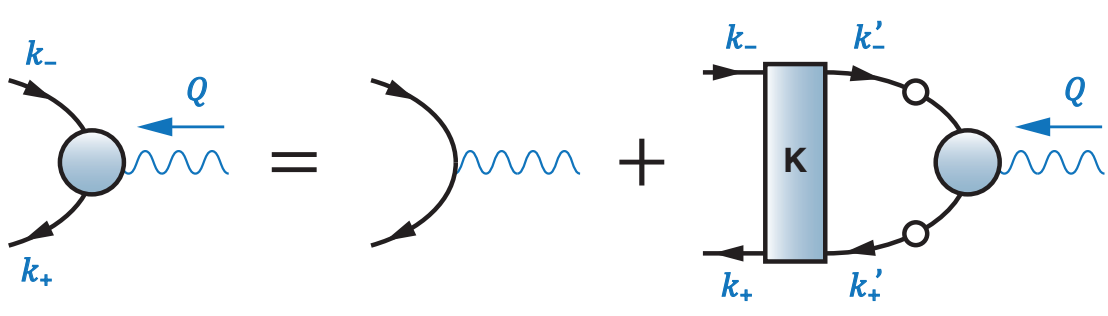
\includegraphics[height=2.7cm, width=10.2cm]{BSE.png}
\end{figure}
\textit{Rainbow-ladder truncation}: approximate the full kernel by
a gluon exchange with an effective interaction given by the Maris-Tandy model 


\end{frame}

\begin{frame}\frametitle{Bethe-Salpeter equation}
	
\begin{equation}
	g(k^2)=Z^2_2\frac{16\pi}{3}\frac{\alpha(k^2)}{k^2}
\end{equation}	

\begin{equation}
\alpha(k^2)=\pi \eta^7 x^2 e^{-\eta^2 x} + \frac{2\pi\gamma_m\left(1-e^{k^2/\Lambda_t^2}\right)}{\ln\left[e^2 - 1 + \left(1 + \frac{k^2}{\Lambda_{QCD}^2}\right)^2\right]}, \qquad x=\frac{k^2}{\Lambda^2}
\end{equation}

The resulting BSE reads explicitly:
\begin{equation}
	\Gamma^\mu(k, Q)=Z_2i\gamma^\mu+\int_{k'}\!\!g(l^2)T^{\alpha\,\beta}_l\gamma^\alpha S(k'_+)\Gamma^\mu(k', Q)S(k'_-)\gamma^\beta
\end{equation}
\end{frame}

\endinput
